\documentclass{article}
\usepackage[utf8]{inputenc}
\usepackage{amsmath}
\usepackage{amssymb}
\usepackage{cancel}
\usepackage{graphicx}
\usepackage{wasysym}
\graphicspath{{Images/}}
\usepackage{chngcntr}
\setlength{\oddsidemargin}{0in}
\setlength{\textwidth}{6.5in}
\setlength{\topmargin}{-0.55in}
\setlength{\textheight}{9in}
\counterwithin{equation}{section}
\pagestyle{empty}

\title{Problem Set 5 (Astrophysics)}
\author{Michael Nameika}
\date{March 2022}

\begin{document}

\maketitle
\begin{center}
    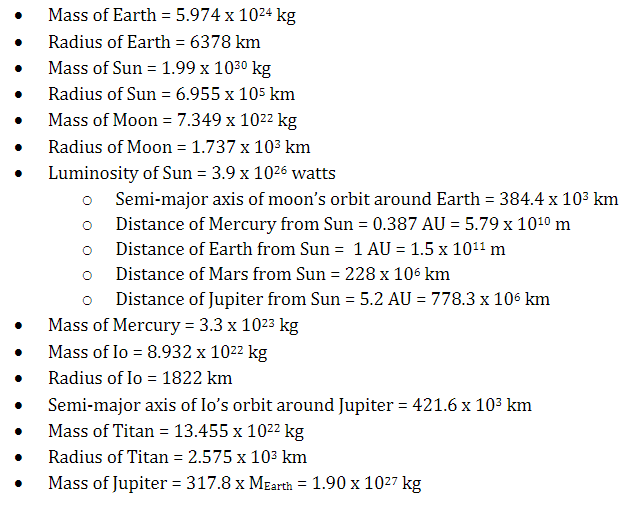
\includegraphics[scale = 0.8]{probset5data.PNG}
\end{center}

\begin{enumerate}
    \item 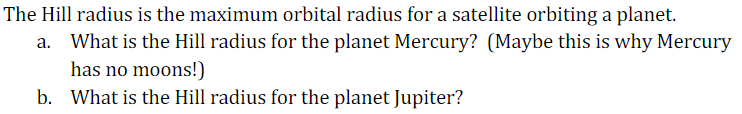
\includegraphics[scale = 0.85]{probset5prob1.PNG}
    
    Recall the formula for the Hill radius:
    \begin{equation}
        r_{Hill} = (\frac{M_{1}}{2M_{2}})^{1/3}r_{1-2}
    \end{equation}
    Where $M_1$ is the mass of the smaller body, $M_2$ is the mass of the larger body, and $r_{1-2}$ is the distance between the two bodies. 
    
    a) From the table given at the beginning of the assignment, we have that 
    \[M_1 = M_{\mercury} = 3.3 \times 10^{23} \:kg\]
    \[M_2 = M_{\bigodot} = 1.99 \times 10^{30} \:kg\]
    \[r_{1-2} = r_{\mercury - \bigodot} = 5.79 \times 10^{10} \:m\]
    Plugging these values into equation (1), we will find
    \[r_{Hill} = (\frac{3.3 \times 10^{23} \:kg}{2*1.99 \times 10^{30} \: kg})^{1/3}(5.79 \times 10^{10} \:m)\]
    \[ \approx 2.52 \times 10^5 \: km\]
    
    b) Also from the table above, we have that 
    \[M_1 = M_{\jupiter} = 1.90 \times 10^{27} \:kg\]
    \[M_2 = M_{\bigodot} = 1.99 \times 10^{30} \:kg\]
    \[r_{1-2} = 7.783 \times 10^8 \:km\]
    Plugging these into equation (1), we get 
    \[r_{Hill} = (\frac{1.90 \times 10^{27} \: kg}{1.99 \times 10^{30} \:kg})^{1/3}(7.783 \times 10^8 \:km)\]
    \[\approx 6.083 \times 10^7 \:km\]
    
    \item 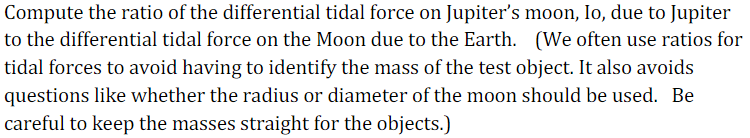
\includegraphics[scale = 0.85]{probset5prob2.PNG}

    Recall that the tidal force on an object due to a massive object on another object with a test mass on its surface is given by
    \begin{equation}
        \Delta F = R_{P}\frac{2GMm}{r_0^3}
    \end{equation}
    Where $R_{P}$ is the radius of the body with the test mass, $M$ is the mass of the body, $m$ is some test mass, and $r_0$ is the center-to-center distance between the massive body and the test mass.
    
    To find the tidal force of Jupiter on Io, using the data in the table above, we will find
    \[\Delta F_{Io} = (1822 \:km)\frac{2G(1.90 \times 10^{27} \: kg)m}{(4.216 \times 10^8 \:m)^3}\]
    And the tidal force of the moon on the Earth:
    \[\Delta F_{Earth} = (6378 \:km) \frac{2G(7.349 \times 10^{22} \:kg)m}{(3.844 \times 10^8 \:m)^3}\]
    And the ratio between the two:
    \[\frac{\Delta F_{Io}}{\Delta F_{Earth}} = \frac{(1822 \:km)\frac{2G(1.90 \times 10^{27} \:kg)m}{(4.216 \times 10^8 \:m)^3}}{(6378 \:km)\frac{2G(7.349 \times 10^22 \:kg)m}{(3.844 \times 10^8 \:m)^3}}\]
    \[ = \frac{(1822)(1.90 \times 10^{27})(3.844 \times 10^8)^3}{(6378)(7.349 \times 10^{22})(4.216 \times 10^8)^3}\]
    \[\approx 5600\]
    So the tidal forces on Io from Jupiter are approximately 5600$\times$ stronger than that of the moon on Earth.
    
    \item 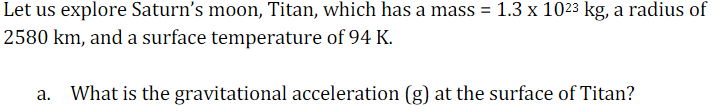
\includegraphics[scale = 0.85]{probset5prob3.PNG} \newline
    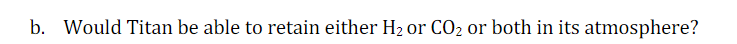
\includegraphics[scale = 0.85]{probset5prob3_1.PNG}
    
    a) Recall that the gravitational acceleration of a body is given by
    \begin{equation}
        a = \frac{GM}{r^2}
    \end{equation}
    Where $M$ is the mass of the body and $r$ is the radius of the body.
    For Titan,
    \[a_{Titan} = \frac{(6.67 \times 10^{-11} \:m^3 kg^{-1} s^{-2})(1.3 \times 10^{23} \:kg)}{(2.58 \times 10^6 \:m)^2}\]
    \[\approx 1.303 \frac{m}{s^2}\]
    So the gravitational acceleration at the surface of Titan is approximately $1.303 \: \frac{m}{s^2}$
    
    b) Recall the formula for the molecular mass that a body can hold:
    \begin{equation}
        \mu \geq 7.1(\frac{T}{1000 \:K})(\frac{M}{M_{\bigodot}})(\frac{R}{R_{\bigodot}})
    \end{equation}
    For Titan, we have
    \[\mu_{Titan} \geq 7.1(\frac{94 \:K}{1000 \:K})(\frac{1.3 \times 10^{23} \:kg}{5.974 \times 10^{24} \:kg})(\frac{2580 \:km}{6378 \:km})\]
    
    \[\approx 0.00587\]
    Since $\mu_{Hydrogen} = 1$, and $\mu_{Titan} \geq 0.00587$, it is safe to assume that Titan will be able to retain both H$_2$ and CO$_2$.
    
    \item 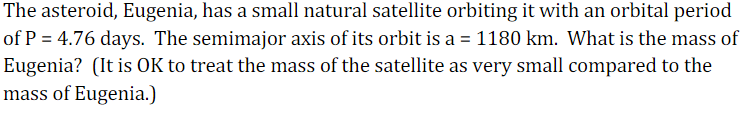
\includegraphics[scale = 0.85]{probset5prob4.PNG}
    
    Recall Kepler's law:
    \begin{equation}
        P^2 \approx \frac{4\pi^2}{Gm}a^3
    \end{equation}
    where $P$ is the period of the object's orbit, $m$ is the parent object's mass and $a$ is the semi-major axis of the orbit.
    
    Solving for $m$ in the above equation, we see that 
    \begin{equation}
        m \approx \frac{4 \pi^2}{GP^2}a^3
    \end{equation}
    So for the data we are given about Eugenia's satellite, we have that
    \[m_{Eugenia} \approx \frac{4\pi^2}{(6.67 \times 10^{-11} \:m^3 \:kg^{-1} \:s^{2})(4.76 * 24 *  60 * 60 s)^2}(1.18 \times 10^6 \:m)\]
    \[\approx 5.75 \times 10^{18} \:kg\]
    So the mass of Eugenia is approximately $5.75 \times 10^{18} \:kg$.
    
    \item 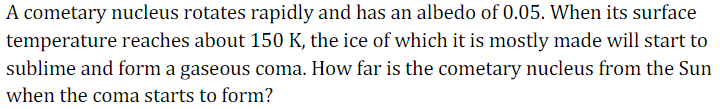
\includegraphics[scale = 0.85]{probset5prob5.PNG}
    
    Recall that we can estimate the temperature of a rapidly rotating object is given by
    \begin{equation}
         T_p = 279 \:K(1-A)^{1/4}(\frac{r}{1 \:AU})^{-1/2}   
    \end{equation}
    
    Solving for $r$ and using the fact that the temperature is $150 \:K$ and the albedo of the comet is $0.05$, we will find that 
    \[r = (\frac{279}{150})^2 (0.95)^{1/2}(1 \:AU)\]
    \[\approx 3.372 \:AU\]
    So a comet's coma will start to form when the comet is approximately $3.372 \:AU$  from the Sun.
    \item 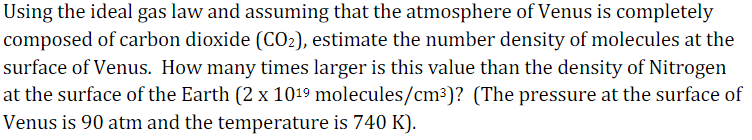
\includegraphics[scale = 0.85]{probset5prob6.PNG}
    
    Recall the ideal gas law:
    \begin{equation}
        PV = NkT
    \end{equation}
    Where $P$ is the pressure, $V$ is the volume, $N$ is the number of molecules, $k$ is Boltzmann's constant ($k = 1.381 \times 10^{-23} \: \frac{Nm}{K}$, and $T$ is the temperature. Plugging in the data given into this equation and solving for $\frac{N}{V}$, we have that 
    \[(\frac{N}{V})_{\venus} = \frac{9.119 \times 10^6 \: \frac{N}{m^2}}{(1.381 \times 10^{-23} \: \frac{Nm}{K})(740 \:K)}\]
    \[\approx 8.92 \times 10^{26} \: \frac{\text{molecules}}{m^3}\]
    \[ = 8.92 \times 10^{20} \: \frac{\text{molecules}}{m^3}\]
    So the number density of molecules of CO$_2$ at the surface of Venus is approximately $8.92 \times 10^{20} \: \frac{\text{molecules}}{m^3}$.
\end{enumerate}


\end{document}
